% !TEX program = xelatex
% =============================================================================
%  Said Bendrioue — Dossier de compétences
%  Mise en page inspirée d'un dossier split navy / or + expériences 2 colonnes.
%  Contenu repris de resume.tex ; lacunes comblées par des formulations
%  recommandées dérivées du profil existant.
%
%  Compilation :
%      xelatex dossier.tex
%  ou  latexmk -xelatex dossier.tex
% =============================================================================
\documentclass[a4paper,10pt]{article}

\usepackage[a4paper,top=18mm,bottom=18mm,left=18mm,right=18mm]{geometry}
\usepackage{fontspec}
\usepackage[french]{babel}
\frenchsetup{AutoSpacePunctuation=false,StandardLists=true}
\usepackage{xcolor}
\usepackage{graphicx}
\usepackage{tikz}
\usepackage{enumitem}
\usepackage{tabularx}
\usepackage{array}
\usepackage{setspace}
\usepackage[
  unicode,
  hidelinks,
  pdflang={fr},
  pdftitle={Said Bendrioue — Dossier de compétences},
  pdfauthor={Said Bendrioue}
]{hyperref}

\pagestyle{empty}
\setlength{\parindent}{0pt}
\setlength{\parskip}{0pt}
\setlength{\emergencystretch}{1.5em}
\raggedright
\frenchspacing

% ----- Couleurs (navy + or du modèle) ----------------------------------------
\definecolor{dcnavy}{HTML}{0F2744}
\definecolor{dcgold}{HTML}{B08B4F}
\definecolor{dcbody}{HTML}{1A1A1A}
\definecolor{dcmuted}{HTML}{4A4A4A}

% ----- Police : Lato (sans-serif du dépôt), repli Source Sans 3 ---------------
\defaultfontfeatures{Ligatures={TeXOff,NoCommon}}
\IfFileExists{./fonts/Lato-Regular.ttf}{%
  \setmainfont{Lato}[
    Path = ./fonts/, Extension = .ttf,
    UprightFont = *-Regular, BoldFont = *-Bold,
    ItalicFont = *-Italic, BoldItalicFont = *-BoldItalic]
}{%
  \setmainfont{SourceSans3}[
    Extension = .otf,
    UprightFont = *-Regular, BoldFont = *-Bold,
    ItalicFont = *-It, BoldItalicFont = *-BoldIt]
}

% ----- Listes ----------------------------------------------------------------
\setlist[itemize]{
  label=\textbullet,
  leftmargin=1.15em,
  labelsep=0.45em,
  itemsep=1.6pt,
  topsep=2.5pt,
  parsep=0pt,
  partopsep=0pt
}

% ----- Helpers de section ----------------------------------------------------
\newcommand{\dcsection}[1]{%
  \par\vspace{3.2mm}%
  {\fontsize{12.5}{14}\selectfont\bfseries\color{dcgold}\MakeUppercase{#1}}\par
  \vspace{2.2mm}%
}

% Titre d'expérience avec filet or jusqu'à la marge droite
\newcommand{\dcexphdr}[1]{%
  \par\vspace{2mm}%
  \noindent
  {\fontsize{12.5}{14}\selectfont\bfseries\color{dcgold}\MakeUppercase{#1}}%
  \hspace{2.5mm}%
  {\color{dcgold}\leaders\hrule height 0.55pt depth -0.15pt\hfill}\hbox{}%
  \par\vspace{5mm}%
}

\newcommand{\dcsub}[1]{%
  \par\vspace{2.8mm}%
  \noindent\textbf{#1}\par
  \vspace{0.6mm}%
}

\newcommand{\dclink}[1]{%
  \par\vspace{2.2mm}%
  \noindent\textit{Lien :} \textit{\href{#1}{#1}}\par
}

\newcommand{\dctech}[2]{%
  \par\vspace{2.4mm}%
  \noindent\textbf{Compétences techniques :}\par
  \vspace{0.8mm}%
  \noindent\textit{Langages et frameworks :} #1\par
  \vspace{0.4mm}%
  \noindent\textit{Technologies et outils :} #2\par
}

\newcommand{\dctechline}[1]{%
  \par\vspace{2.4mm}%
  \noindent\textbf{Technologies :} #1\par
}

% Entrée expérience : colonne gauche (meta) + colonne droite (détail)
\newlength{\dcleftw}
\setlength{\dcleftw}{38mm}
\newlength{\dcgap}
\setlength{\dcgap}{7mm}
\newcommand{\dcexperience}[2]{%
  \par\noindent
  \begin{minipage}[t]{\dcleftw}
    \raggedright
    #1
  \end{minipage}%
  \hspace{\dcgap}%
  \begin{minipage}[t]{\dimexpr\textwidth-\dcleftw-\dcgap\relax}
    \raggedright
    \color{dcbody}#2
  \end{minipage}%
  \par
}

\newcommand{\dcjob}[3]{%
  {\fontsize{11}{13}\selectfont\bfseries\color{dcnavy}#1}\par
  \vspace{0.6mm}%
  {\fontsize{10.5}{12.5}\selectfont\bfseries\color{dcnavy}#2}\par
  \vspace{0.8mm}%
  {\fontsize{8.5}{10.5}\selectfont\itshape\color{dcmuted}(#3)}\par
}

\newcommand{\dcrule}{%
  \par\vspace{5mm}%
  {\color{dcgold}\hrule height 0.55pt}\par
  \vspace{5mm}%
}

\newcommand{\dcfooter}[1]{%
  \vfill
  \noindent{\footnotesize\color{dcmuted}#1}%
}

% Timeline formations (années de fin, comme le modèle)
\newcommand{\dctimeline}{%
  \vspace{2mm}%
  \noindent
  \begin{tikzpicture}[x=\textwidth, y=1cm]
    \draw[dcgold, line width=2.4pt] (0.06,0) -- (0.94,0);
    % 2017 — Licence (année, diplôme, école sous le point)
    \fill[dcnavy] (0.30,0) circle (3.6pt);
    \node[anchor=north, align=center, font=\small\bfseries, text=dcbody]
      at (0.30,-0.32) {2017};
    \node[anchor=north, align=center, font=\footnotesize\bfseries, text=dcbody]
      at (0.30,-0.85) {Licence Mathématiques\\et informatique};
    \node[anchor=north, align=center, font=\footnotesize\itshape, text=dcbody]
      at (0.30,-1.65) {Université Abdelmalek Essaâdi};
    % 2019 — Master
    \fill[dcnavy] (0.70,0) circle (3.6pt);
    \node[anchor=north, align=center, font=\small\bfseries, text=dcbody]
      at (0.70,-0.32) {2019};
    \node[anchor=north, align=center, font=\footnotesize\bfseries, text=dcbody]
      at (0.70,-0.85) {Master Informatique\\appliquée offshoring};
    \node[anchor=north, align=center, font=\footnotesize\itshape, text=dcbody]
      at (0.70,-1.65) {Université Mohammed V\\de Rabat};
  \end{tikzpicture}%
  \vspace{28mm}%
}

\begin{document}
\color{dcbody}

% =============================================================================
% PAGE 1 — Couverture
% =============================================================================
\newgeometry{margin=0pt}
\begin{tikzpicture}[remember picture, overlay]
  % Split navy / blanc
  \fill[dcnavy] (current page.south west) rectangle
    ([xshift=0.42\paperwidth]current page.north west);
  % Titre collé au bord droit de la colonne navy, centré verticalement
  \node[
    anchor=east,
    align=right,
    font=\fontsize{20}{26}\selectfont\bfseries,
    text=white,
    inner sep=0pt
  ] at ([xshift=0.395\paperwidth]current page.west)
  {DOSSIER DE\\COMPÉTENCES};

  % Bloc identité (colonne blanche), moitié basse comme le modèle
  \node[
    anchor=north west,
    inner sep=0pt,
    text width=0.44\paperwidth
  ] at ([xshift=0.48\paperwidth, yshift=-0.42\paperheight]current page.north west) {
    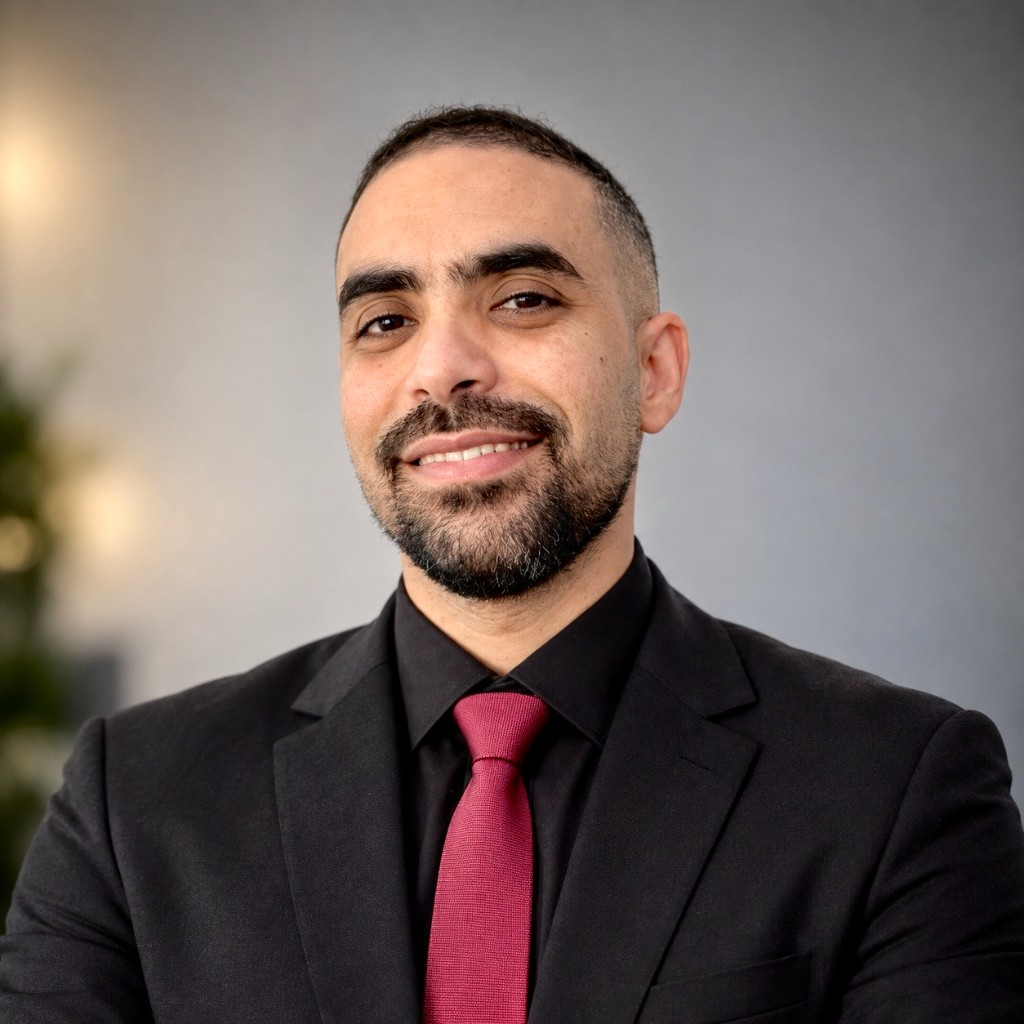
\includegraphics[width=44mm]{profile.jpg}\\[4.5mm]
    {\fontsize{11}{13}\selectfont\bfseries\color{dcnavy}BENDRIOUE Said}\\[2.4mm]
    {\fontsize{17}{20}\selectfont\bfseries\color{dcgold}Développeur Fullstack}\\[0.2mm]
    {\fontsize{17}{20}\selectfont\bfseries\color{dcgold}Java/Angular}\\[1.4mm]
    {\fontsize{12.5}{15}\selectfont\bfseries\color{dcgold}8 années d'expérience}\\[5.5mm]
    {\fontsize{8.5}{11.2}\selectfont\color{dcnavy}%
      \href{tel:+33749320616}{+33~7~49~32~06~16}\\
      \href{mailto:bendrioue@gmail.com}{bendrioue@gmail.com}\\
      \href{https://www.linkedin.com/in/said-bendrioue}{linkedin.com/in/said-bendrioue}\\
      \href{https://saidbendrioue.github.io/portfolio}{saidbendrioue.github.io/portfolio}
    }
  };
\end{tikzpicture}
\clearpage
\restoregeometry

% =============================================================================
% PAGE 2 — À propos / Formations / Compétences / Références
% =============================================================================
\dcsection{À propos}

Fullstack Senior Java/Angular et Scrum Master (8~ans), systèmes critiques~:
fiabilité, sécurité, conformité (vote électronique, données financières,
bancaire). Cible~: CDI Nice~/ hybride.

\vspace{2.5mm}
\noindent J'ai collaboré avec des entreprises comme~:
\begin{itemize}
  \item Docaposte
  \item La Poste Groupe
  \item Crédit Agricole Technologies et Services
  \item Bouygues Construction IT
\end{itemize}

\vspace{1.5mm}
\noindent Je suis en mesure de~:
\begin{itemize}
  \item Concevoir et développer des applications fullstack Java~/ Angular
  \item Animer une équipe Agile en tant que Scrum Master
  \item Migrer et moderniser des SI (Oracle~$\rightarrow$~PostgreSQL, legacy~$\rightarrow$~stack moderne)
  \item Sécuriser APIs et données sensibles (JWT, RGPD, contextes critiques)
  \item Industrialiser les livraisons (Docker, Kubernetes, CI/CD)
  \item Garantir la qualité logicielle (JUnit, Mockito, SonarQube)
  \item Intervenir sur des systèmes réglementés (vote, bancaire, social)
\end{itemize}

\dcsection{Formations}
\dctimeline

\noindent
\begin{minipage}[t]{0.62\textwidth}
\dcsection{Compétences}
\vspace{-1mm}
\noindent\textbf{Langages :} Java~17, TypeScript, SQL\\[1.2mm]
\noindent\textbf{Frameworks \& bibliothèques :} Spring Boot, Spring Security, Hibernate,
Angular, RxJS, NgRx\\[1.2mm]
\noindent\textbf{Architectures \& concepts :} API REST, Microservices, JWT, Kafka\\[1.2mm]
\noindent\textbf{Data :} PostgreSQL, Oracle, Liquibase, Ora2Pg\\[1.2mm]
\noindent\textbf{Outils \& environnements :} Docker, Kubernetes, GitLab CI, Jenkins, Git, Maven,
SonarQube\\[1.2mm]
\noindent\textbf{Méthodologies \& gestion d'équipe :} Scrum Master, Jira, TDD
\end{minipage}%
\hfill
\begin{minipage}[t]{0.32\textwidth}
\dcsection{Autres}
\vspace{-1mm}
\noindent Anglais : professionnel\\[1.2mm]
\noindent Français : courant\\[1.2mm]
\noindent Arabe : bilingue\\[1.2mm]
\noindent Nice~/ hybride
\end{minipage}

\vspace{2mm}
\dcsection{Références}
{\small\itshape\color{dcgold}Informations des contacts disponibles sur demande.}

\dcfooter{2}
\clearpage

% =============================================================================
% PAGE 3 — Expériences (Docaposte / e-Vote)
% =============================================================================
\dcexphdr{Expériences}

\dcexperience{%
  \dcjob{Fullstack Java/Angular\\Scrum Master}{Docaposte — e-Vote (Voxaly)}{12/2025 – 08/2026}
}{%
  Plateforme de vote électronique pour organisations (échelle~: $\sim$165~000 électeurs,
  2~000+ orgs). Mission fullstack et animation Scrum sur le cycle de vie des candidatures
  et le contrôle des pièces électorales.

  \dcsub{Chiffres clé :}
  \begin{itemize}
    \item $\sim$165~000 électeurs et 2~000+ organisations
    \item Vélocité d'équipe \textbf{+15~\%} via animation Scrum / Jira
  \end{itemize}

  \dcsub{Composition d'équipe :}
  \begin{itemize}
    \item Équipe produit Agile (PO, développeurs, QA) — animation Scrum Master
  \end{itemize}

  \dcsub{Mes responsabilités :}
  \begin{itemize}
    \item Cycle de vie des candidatures (création $\rightarrow$ validation/rejet) avec
          traçabilité des statuts et dates
    \item Règles et contrôles des pièces électorales (DIC, profession de foi, logo, signature)
    \item Exports CSV/PDF/ZIP sync et async pour le suivi opérationnel
    \item Habilitations par profil (OS, valideur, admin), robustesse backend et notifications e-mail
    \item Animation Scrum et pilotage Jira
  \end{itemize}

  \dcsub{Compétences démontrées :}
  \begin{itemize}
    \item Maîtrise fullstack sur un SI critique réglementé
    \item Capacité à faire progresser la vélocité d'une équipe Agile
    \item Rigueur sur traçabilité, habilitations et fiabilité métier
  \end{itemize}

  \dclink{https://saidbendrioue.github.io/portfolio}
  \dctech{Java, Spring Boot, Angular, TypeScript, RxJS, NgRx}%
         {API REST, JWT, GitLab CI, Jira, Git}
}

\dcfooter{3}
\clearpage

% =============================================================================
% PAGE 4 — EAS + Bilans
% =============================================================================
\dcexperience{%
  \dcjob{Fullstack Java/Angular\\Scrum Master}{Docaposte — EAS (La Poste)}{08/2024 – 05/2025}
}{%
  Portail B2E de prestations sociales pour La Poste~: dépôt, instruction et validation
  des dossiers, avec persistance IBAN / identifiants RH et contrôles RGPD.

  \dcsub{Chiffres clé :}
  \begin{itemize}
    \item Portail national B2E prestations sociales La Poste
    \item Sprints de 2~semaines, backlog co-construit avec le PO
  \end{itemize}

  \dcsub{Composition d'équipe :}
  \begin{itemize}
    \item Équipe Agile (PO, développeurs, QA) — rôle Scrum Master
  \end{itemize}

  \dcsub{Mes responsabilités :}
  \begin{itemize}
    \item API REST Spring Boot / JWT (dépôt $\rightarrow$ instruction $\rightarrow$ validation)
    \item SPA Angular (RxJS, NgRx) pour agents et gestionnaires
    \item GED et contrôles RGPD (chiffrement, consentements, droit à l'effacement)
    \item Facilitation Scrum~; déploiement Docker / CI-CD sur hébergement souverain
  \end{itemize}

  \dcsub{Compétences démontrées :}
  \begin{itemize}
    \item Expertise fullstack sur données RH / sociales sensibles
    \item Animation Agile de bout en bout (backlog, cérémonies, livraison)
    \item Intégration conformité RGPD dans le cycle de développement
  \end{itemize}

  \dctech{Java, Spring Boot, Angular, TypeScript, RxJS, NgRx}%
         {JWT, Docker, CI/CD, cloud souverain, Git}
}

\dcrule

\dcexperience{%
  \dcjob{Backend / Data}{Docaposte — Bilans Service}{05/2025 – 11/2025}
}{%
  Migration Oracle~$\rightarrow$~PostgreSQL du service Bilans~: objets SQL, conteneurisation
  et industrialisation CI/CD, avec accompagnement recette / MEP.

  \dcsub{Chiffres clé :}
  \begin{itemize}
    \item Migration complète Oracle~$\rightarrow$~PostgreSQL (Ora2Pg)
    \item Base PostgreSQL conteneurisée et pipeline CI/CD
  \end{itemize}

  \dcsub{Mes responsabilités :}
  \begin{itemize}
    \item Migration des objets SQL via Ora2Pg
    \item Conteneurisation PostgreSQL sous Docker
    \item Industrialisation CI/CD et accompagnement recette / MEP
  \end{itemize}

  \dcsub{Compétences démontrées :}
  \begin{itemize}
    \item Capacité à migrer un SI data critique sans rupture
    \item Industrialisation et accompagnement métier jusqu'à la MEP
  \end{itemize}

  \dctechline{Oracle, PostgreSQL, Ora2Pg, SQL, Docker, CI/CD, Git}
}

\dcfooter{4}
\clearpage

% =============================================================================
% PAGE 5 — MFS + Timbre électronique
% =============================================================================
\dcexperience{%
  \dcjob{Fullstack\\Scrum Master}{Docaposte — Maison France Services}{08/2023 – 07/2024}
}{%
  Plateforme nationale pour les conseillers France Services~: APIs Spring Boot,
  formulaires dynamiques Angular, déploiement cloud souverain et facilitation Scrum.

  \dcsub{Chiffres clé :}
  \begin{itemize}
    \item Plateforme pour $\sim$8~000 conseillers France Services
    \item Mission au sein de Docaposte (août~2023 – août~2026)
  \end{itemize}

  \dcsub{Mes responsabilités :}
  \begin{itemize}
    \item Développement d'APIs Spring Boot et formulaires dynamiques Angular
    \item Déploiement sur cloud souverain
    \item Facilitation Scrum de l'équipe
  \end{itemize}

  \dcsub{Compétences démontrées :}
  \begin{itemize}
    \item Livraison fullstack à grande échelle (milliers d'utilisateurs)
    \item Double casquette technique / Scrum Master
  \end{itemize}

  \dctech{Java, Spring Boot, Angular}%
         {Cloud souverain, Scrum, Jira, Git}
}

\dcrule

\dcexperience{%
  \dcjob{Backend Java}{La Poste Groupe — Timbre électronique}{01/2023 – 08/2023}
}{%
  Microservices Spring Boot pour la commande, la génération et la vérification
  temps réel des identifiants de timbres électroniques, avec traçabilité vers le SI
  logistique.

  \dcsub{Chiffres clé :}
  \begin{itemize}
    \item Vérification temps réel des identifiants de timbres
    \item Intégration SI logistique via API REST et Kafka
  \end{itemize}

  \dcsub{Mes responsabilités :}
  \begin{itemize}
    \item Développement microservices Spring Boot (commande, génération, vérification)
    \item API REST et Kafka pour fiabilité / traçabilité
    \item Contrôles anti-fraude et règles tarifaires
    \item Tests JUnit / Robot Framework~; contribution CI/CD avec métier, QA et DevOps
  \end{itemize}

  \dcsub{Compétences démontrées :}
  \begin{itemize}
    \item Conception de microservices fiables en environnement logistique
    \item Collaboration transverse métier / QA / DevOps
  \end{itemize}

  \dctechline{Java, Spring Boot, Microservices, Kafka, API REST, JUnit, Robot Framework, CI/CD, Git}
}

\dcfooter{5}
\clearpage

% =============================================================================
% PAGE 6 — Crédit Agricole + Bouygues
% =============================================================================
\dcexperience{%
  \dcjob{Fullstack Java/Angular}{Crédit Agricole Technologies et Services}{05/2022 – 12/2022}
}{%
  Parcours national de changement d'adresse~: propagation sync/async vers le SI bancaire,
  validation postale et piste d'audit réglementaire.

  \dcsub{Chiffres clé :}
  \begin{itemize}
    \item Parcours omnicanal national (réseau bancaire)
    \item Qualité renforcée via gates SonarQube
  \end{itemize}

  \dcsub{Mes responsabilités :}
  \begin{itemize}
    \item Développement fullstack du parcours de changement d'adresse
    \item Propagation sync/async vers le SI bancaire
    \item Validation postale et piste d'audit réglementaire
    \item Tests JUnit / Mockito et gates SonarQube
  \end{itemize}

  \dcsub{Compétences démontrées :}
  \begin{itemize}
    \item Maîtrise des contraintes bancaires et d'audit
    \item Qualité logicielle et industrialisation des contrôles
  \end{itemize}

  \dctechline{Java, Angular, JUnit, Mockito, SonarQube, Git}
}

\dcrule

\dcexperience{%
  \dcjob{Fullstack Java/Angular}{Bouygues Construction IT — e-Doc (GED)}{07/2019 – 04/2022}
}{%
  Migration progressive d'une GED chantier Java~6/GWT vers Java~11/Angular~:
  modules plans (versioning), workflows de visas et application unifiée pour les chantiers.

  \dcsub{Chiffres clé :}
  \begin{itemize}
    \item Migration multi-années Java~6/GWT $\rightarrow$ Java~11/Angular
    \item Application unifiée déployée sur les chantiers
  \end{itemize}

  \dcsub{Mes responsabilités :}
  \begin{itemize}
    \item Migration progressive du socle technique
    \item Modules plans (versioning) et workflows de visas
    \item Unification de l'application GED pour les chantiers
  \end{itemize}

  \dcsub{Compétences démontrées :}
  \begin{itemize}
    \item Conduite de modernisation applicative sur le long terme
    \item Expertise fullstack Java / Angular en contexte métier BTP
  \end{itemize}

  \dctechline{Java~11, Angular, GWT (legacy), Git}
}

\dcfooter{6}

\end{document}
